% =====================================================================
%  qgmutualinfo.tex -- A. J. Larkoski, J. Thaler, W. J. Waalewijn,
%  "Gaining (Mutual) Information about Quark/Gluon Discrimination",
%  JHEP 11 (2014) 129 [arXiv:1408.3122], recast in the notation of
%  chapters/intro.tex and chapters/angularities.tex.
%
%  WHERE IT GOES: as a section either at the end of Sec. 1.4
%  (sec:partonShower), after jetportrait.tex, or as the opening
%  theory section of Ch. \ref{ch:angularities}.  It is written as a
%  \section with \subsections, matching jetportrait.tex.
%
%  NOTATION MAP -- paper -> thesis:
%    \lambda^\kappa_\beta   -> same symbol, Eq. \ref{eq:LambdaKappaBeta}
%    e_\beta = \lambda^1_\beta -> written \lambda^1_\beta throughout
%    C_i (C_F, C_A)         -> \mathbf{Q}_i^2, intro.tex Sec. 1.4.2
%    \theta_i = R_i/R_0     -> \Delta R_{const,jet}/R
%    \Sigma_i(e)            -> \Sigma_i(\lambda), same
%    their \beta_0, \beta_1 -> the thesis' \beta_0 (eq:RGEquation)
%    P_{i\to ig}(z)         -> \hat{P}_{gi}(z), Table \ref{tab:splitfns}
%
%  LABELS ASSUMED TO EXIST (all currently live):
%    ch:intro, ch:angularities, sec:partonShower, subsec:dglap,
%    sec:coherentPartonBranching, tab:splitfns, eq:antennaSplitXSec,
%    eq:angularOrdering, eq:coherentSudakov, eq:runningCouplingLambda,
%    eq:RGEquation, eq:LambdaKappaBeta, fig:GroomingAndRg
%
%  IF jetportrait.tex IS UNCOMMENTED in intro.tex, three derivations
%  below become one-line callbacks instead:
%    eq:qgmiLLsudakov  == jetportrait's eq:angularitySudakov
%    the (u,v) plane   == jetportrait's Eq. (angularityDef), 2nd line
%    9/4 and delta_g   == jetportrait's eq:casimirRatio, eq:swWidth
%  I have kept them self-contained here, with a pointer, so the file
%  compiles against intro.tex as it stands today.  Labels are all
%  prefixed eq:qgmi.../fig:qgmi... so nothing collides with
%  jetportrait.tex or qgjets.tex.
%
%  BIBTEX: \cite{Larkoski_2014} already resolves -- but thesis.bib
%  contains THREE identical Larkoski_2014 entries (lines 101, 268,
%  3092).  BibTeX takes the first and warns on the rest; worth
%  deduplicating at some point.  Not touched here.
% =====================================================================

\section{Quark--gluon discrimination as an information problem}
\label{sec:qgmi}

Chapter~\ref{ch:intro} ended with a cascade whose every emission rate is
proportional to the squared colour charge \(\mathbf{Q}_i^2\) of whatever is
radiating. That single fact is the whole of quark--gluon discrimination at lowest
order, and it is also its ceiling. The purpose of this section is to make that
statement quantitative, following Larkoski, Thaler and
Waalewijn~\cite{Larkoski_2014}, who ask two questions that the cascade alone does
not answer: \emph{how much} separation does \(\mathbf{Q}_g^2/\mathbf{Q}_q^2=9/4\)
actually buy, and \emph{what has to be true} of an observable for it to do better.
The answers are, respectively, about a tenth of one bit, and that the observable
must resolve something in the jet other than its overall colour charge.

\subsection{The observable family, in the variables of Chapter~\ref{ch:intro}}
\label{subsec:qgmiFamily}

The paper's discriminants are exactly the generalized angularities of
Eq.~\ref{eq:LambdaKappaBeta},
\begin{equation}
	\lambda^\kappa_\beta = \sum_{c\,\in J} z_c^\kappa\,\theta_c^\beta ,
	\qquad
	z_c = \frac{p_{\mathrm{T},c}}{\sum_{c^\prime\in J}p_{\mathrm{T},c^\prime}} ,
	\qquad
	\theta_c = \frac{\Delta R_{c}}{R} ,
	\label{eq:qgmiAngularity}
\end{equation}
with \(0\le z_c,\theta_c\le1\) and both exponents non-negative. A single
two-parameter family contains most of the observables the quark--gluon literature
uses, at the four corners of Fig.~\ref{fig:qgmiLambdaSpace}: \(\lambda^0_0\) is
constituent multiplicity, \(\lambda^2_0\) is \(p_T^D\), \(\lambda^1_1\) is the jet
width (girth, broadening), and \(\lambda^1_2\) is thrust, i.e.\ jet mass squared
over energy squared. Raising \(\beta\) weights wide-angle radiation, raising
\(\kappa\) weights hard constituents; \(\beta\) reaches into the cascade's angular
ordering and \(\kappa\) into its energy sharing, and these are the two independent
handles Sec.~\ref{sec:coherentPartonBranching} provides.

\begin{figure}[htbp]
	\centering
	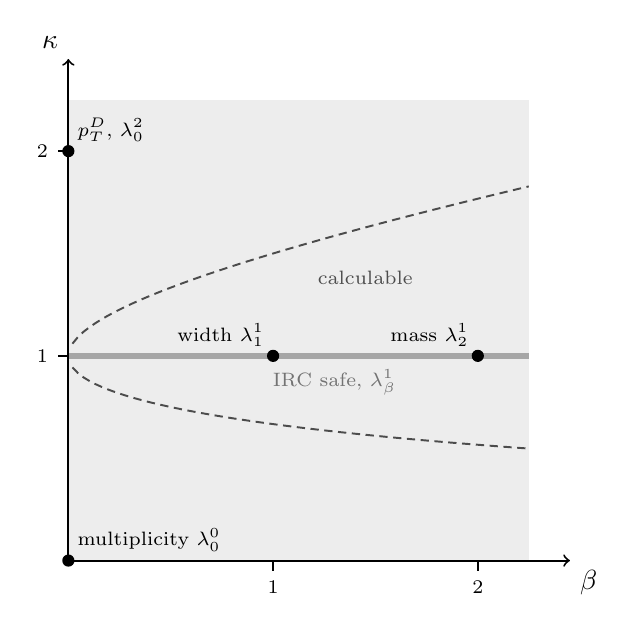
\begin{tikzpicture}[x=2.6cm, y=2.6cm, line width=0.7pt]
		\fill[black!7] (0,0) rectangle (2.25,2.25);
		% IRC-safe line kappa = 1
		\draw[line width=2.2pt, black!35] (0,1) -- (2.25,1);
		\node[black!55, font=\scriptsize] at (1.30,0.87)
		{IRC safe, \(\lambda^1_\beta\)};
		\draw[->] (0,0) -- (2.45,0) node[below right] {\(\beta\)};
		\draw[->] (0,0) -- (0,2.45) node[above left] {\(\kappa\)};
		\foreach \i in {1,2} {
			\draw (\i,0) -- (\i,-0.05) node[below] {\scriptsize\(\i\)};
			\draw (0,\i) -- (-0.05,\i) node[left] {\scriptsize\(\i\)};
		}
		\foreach \p/\l/\a in {%
			{0,0}/{multiplicity \(\lambda^0_0\)}/{above right},
			{0,2}/{\(p_T^D\), \(\lambda^2_0\)}/{above right},
			{1,1}/{width \(\lambda^1_1\)}/{above left},
			{2,1}/{mass \(\lambda^1_2\)}/{above left}} {
			\fill (\p) circle (2.2pt);
			\node[\a, font=\scriptsize, inner sep=3pt] at (\p) {\l};
		}
		% edge of the calculable region: 6(1-kappa)^2 = beta*kappa, i.e.
		% kappa = [(12+beta) +- sqrt((12+beta)^2-144)]/12
		\draw[densely dashed, black!70] plot[domain=0.02:2.25, samples=80]
		(\x, {((12+\x) - sqrt((12+\x)*(12+\x)-144))/12});
		\draw[densely dashed, black!70] plot[domain=0.02:2.25, samples=80]
		(\x, {((12+\x) + sqrt((12+\x)*(12+\x)-144))/12});
		\node[font=\scriptsize, black!70] at (1.45,1.38) {calculable};
	\end{tikzpicture}
	\caption[The space of generalized angularities]{%
		The \((\beta,\kappa)\) plane of Eq.~\ref{eq:qgmiAngularity}. The line
		\(\kappa=1\) holds the IRC safe angularities; the four marked points are the
		observables in common use. Inside the dashed contour,
		\(\beta\kappa/(1-\kappa)^2>6\) of Eq.~\ref{eq:qgmiBarrier}, the distribution
		is calculable from the cascade with a single non-perturbative number; outside
		it, an entire non-perturbative function is needed. Redrawn from
		Ref.~\cite{Larkoski_2014}.}
	\label{fig:qgmiLambdaSpace}
\end{figure}

Two features of Eq.~\ref{eq:qgmiAngularity} carry consequences that are easy to
miss and that both bear on Chapter~\ref{ch:angularities}.

\paragraph{Infrared and collinear safety sits at \(\kappa=1\) only.} Splitting a
constituent of momentum fraction \(z\) into two collinear pieces \(z_1+z_2=z\)
changes \(\sum z_c^\kappa\) by \(z_1^\kappa+z_2^\kappa-z^\kappa\), which vanishes
only for \(\kappa=1\). The \(\beta>0\) suppression handles the collinear region at
the \emph{jet axis} but not collinear splittings of a wide-angle constituent, so
\(\kappa\neq1\) is collinear unsafe everywhere in \(\beta\). This is the same
statement as the one made after Eq.~\ref{eq:LambdaKappaBeta}: restricting the sum
to charged tracks is a \(\kappa\)-like reweighting and costs IRC safety.
Sec.~\ref{subsec:qgmiUnsafe} is the machinery that buys it back.

\paragraph{The axis must be recoil-free.} Ref.~\cite{Larkoski_2014} measures
\(\Delta R_c\) to the \emph{winner-take-all} axis, not to the jet momentum axis.
The distinction is invisible at \(\beta\ge1\) but not below: with a momentum axis, a
single hard wide-angle emission displaces the axis itself, so \(\lambda^\kappa_\beta\)
measures the recoil of the initiating parton rather than the radiation pattern about
it, and the resummation acquires a second, spurious source of logarithms. Every
analytic statement below assumes a recoil-free axis. The measurement in
Chapter~\ref{ch:angularities} uses the standard jet axis, so the calculations quoted
here are a guide to the physics rather than a prediction to be overlaid on the data
--- unless the axis is changed.

The one kinematic picture used throughout is the cascade's own. Eq.~\ref{eq:antennaSplitXSec}
in the soft-collinear limit gives a single emitter the emission density
\begin{equation}
	dn = \frac{2\alpha_s\mathbf{Q}_i^2}{\pi}\frac{dz}{z}\frac{d\theta}{\theta}
	= \frac{2\alpha_s\mathbf{Q}_i^2}{\pi}\,du\,dv ,
	\qquad
	u = \ln\frac{1}{z} ,
	\qquad
	v = \ln\frac{1}{\theta} ,
	\label{eq:qgmiLundPlane}
\end{equation}
uniform on the quadrant \(u,v>0\) with a density set entirely by \(\mathbf{Q}_i^2\).
An emission contributes \(z^\kappa\theta^\beta = e^{-(\kappa u+\beta v)}\) to
Eq.~\ref{eq:qgmiAngularity}, so \(\lambda^\kappa_\beta>\lambda\) requires an emission
below the straight line \(\kappa u+\beta v=\ln(1/\lambda)\). Every result in this
section is a statement about that line and about the uniform density it cuts.

\subsection{Truth overlap: the right way to score a discriminant}
\label{subsec:qgmiMI}

The paper's organising quantity is the \emph{mutual information} between two
variables,
\begin{equation}
	I(A;B) = \int da\,db\;p(a,b)\log_2\frac{p(a,b)}{p(a)p(b)}
	= H(A)+H(B)-H(A,B) ,
	\label{eq:qgmiMIdef}
\end{equation}
with \(H\) the Shannon entropy, \(H(A)=-\sum_a p(a)\log_2p(a)\). Written the second
way it is manifestly the overlap area of two sets in Fig.~\ref{fig:qgmiVenn}:
\(H(A)\) and \(H(B)\) are the number of bits each variable carries, \(H(A,B)\) the
number the two carry together, and \(I(A;B)\) the bits they share. It vanishes iff
\(a\) and \(b\) are independent.

Now let \(T\) be the jet's flavour, \(t=0\) for a quark and \(t=1\) for a gluon, and
take a sample that is half of each, so that \(H(T)=1\): there is exactly one bit of
truth to be recovered, no matter how many bits an observable carries in total. The
\emph{truth overlap} of an observable is its mutual information with that bit,
\begin{equation}
	I(T;A) = \int d\lambda\left[
	\frac{p_q(\lambda)}{2}\log_2\frac{p_q(\lambda)}{p_{\rm tot}(\lambda)}
	+ \frac{p_g(\lambda)}{2}\log_2\frac{p_g(\lambda)}{p_{\rm tot}(\lambda)}\right] ,
	\qquad
	p_{\rm tot} = \frac{p_q+p_g}{2} ,
	\label{eq:qgmiTruthOverlap}
\end{equation}
bounded by \(0\le I(T;A)\le H(T)=1\), zero for two identical distributions and one
for two that do not overlap. It plays the role a ROC curve plays in an experimental
paper --- and indeed if one observable's ROC curve is everywhere better than
another's, its truth overlap is strictly larger, so nothing is lost by the change of
language --- but unlike a ROC curve it is a single number with a closed-form
integral, which is what makes the analytic study below possible.

\begin{figure}[htbp]
	\centering
	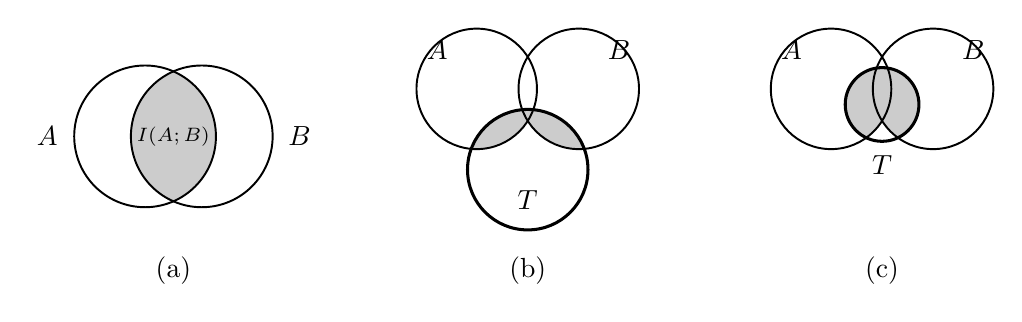
\begin{tikzpicture}[line width=0.7pt, scale=0.90,
		lens/.style={fill=black!20}]
		% ---- (a) I(A;B) ----
		\begin{scope}[yshift=-0.15cm]
			\begin{scope}
				\clip (-0.40,0) circle (1.00);
				\fill[lens] (0.40,0) circle (1.00);
			\end{scope}
			\draw (-0.40,0) circle (1.00);
			\draw (0.40,0) circle (1.00);
			\node at (-1.78,0) {\(A\)};
			\node at (1.78,0) {\(B\)};
			\node[font=\scriptsize] at (0,0) {\(I(A;B)\)};
			\node at (0,-1.90) {(a)};
		\end{scope}
		% ---- (b) complementary: A and B reach T in two different places ----
		\begin{scope}[xshift=5.0cm]
			\begin{scope}
				\clip (0,-0.62) circle (0.85);
				\fill[lens] (-0.72,0.52) circle (0.85);
				\fill[lens] (0.72,0.52) circle (0.85);
			\end{scope}
			\draw (-0.72,0.52) circle (0.85) node[above left=0.24cm] {\(A\)};
			\draw (0.72,0.52) circle (0.85) node[above right=0.24cm] {\(B\)};
			\draw[line width=1.1pt] (0,-0.62) circle (0.85);
			\node at (0,-1.05) {\(T\)};
			\node at (0,-2.05) {(b)};
		\end{scope}
		% ---- (c) redundant: same A and B, T moved onto their overlap ----
		\begin{scope}[xshift=10.0cm]
			\begin{scope}
				\clip (0,0.30) circle (0.52);
				\fill[lens] (-0.72,0.52) circle (0.85);
				\fill[lens] (0.72,0.52) circle (0.85);
			\end{scope}
			\draw (-0.72,0.52) circle (0.85) node[above left=0.24cm] {\(A\)};
			\draw (0.72,0.52) circle (0.85) node[above right=0.24cm] {\(B\)};
			\draw[line width=1.1pt] (0,0.30) circle (0.52);
			\node at (0,-0.55) {\(T\)};
			\node at (0,-2.05) {(c)};
		\end{scope}
	\end{tikzpicture}
	\caption[Mutual information and truth overlap]{%
		(a) Mutual information \(I(A;B)\), Eq.~\ref{eq:qgmiMIdef}, as the shared area
		of two variables in information space. (b) and (c): the observables \(A\) and
		\(B\) are drawn identically in the two panels, so their correlation
		\(I(A;B)\) is the same; only the truth bit \(T\) has moved. Shaded is the
		joint truth overlap \(I(T;A,B)\), the part of \(T\) reached by either
		observable. In (b) the two reach \(T\) in different places and the shaded
		region is much larger than the part either reaches alone, so combining them
		gains; in (c) they reach it in the same place, the shaded region is barely
		larger than either lobe, and combining them gains nothing. Correlation
		between observables and complementarity for discrimination are therefore
		separate questions. After Ref.~\cite{Larkoski_2014}.}
	\label{fig:qgmiVenn}
\end{figure}

The distinction the paper is built around is between \(I(A;B)\) and
\begin{equation}
	I(T;A,B) = H(T) + H(A,B) - H(T,A,B)
	\;\geq\; \max\left\{I(T;A),\,I(T;B)\right\} ,
	\label{eq:qgmiJoint}
\end{equation}
the truth overlap of the \emph{pair}. The first measures whether two observables are
correlated; the second measures whether their correlation, or lack of it, is of any
use. Figure~\ref{fig:qgmiVenn}(b) and (c) are drawn with identical \(I(A;B)\) and
identical individual truth overlaps and different \(I(T;A,B)\). This resolves a
standing puzzle in the substructure literature, where two variables are repeatedly
found to be weakly correlated and yet to gain nothing when combined: they are
uncorrelated in the bits that carry no flavour information and redundant in the bits
that do. The useful figure of merit is therefore the \emph{gain}
\begin{equation}
	\Delta I(T;A\to A,B) \equiv I(T;A,B) - \max\left\{I(T;A),I(T;B)\right\} ,
	\label{eq:qgmiGain}
\end{equation}
not the correlation coefficient.

\subsection{Casimir scaling, and why it caps the answer near a tenth of a bit}
\label{subsec:qgmiCasimir}

Call an observable \emph{Casimir scaling} if its cumulative distributions --- the
fraction of jets with the observable below \(\lambda\) --- take the form
\begin{equation}
	\Sigma_q(\lambda) = e^{-C_F\,r(\lambda)} ,
	\qquad
	\Sigma_g(\lambda) = e^{-C_A\,r(\lambda)}
	= \left[\Sigma_q(\lambda)\right]^{C_A/C_F} ,
	\label{eq:qgmiCasimir}
\end{equation}
for \emph{any} monotonic \(r\). The quark and gluon curves differ by a power, and by
nothing else: the observable has seen the jet's colour charge and no other property
of it. Equation~\ref{eq:qgmiCasimir} is the generic outcome of the cascade, because
Eq.~\ref{eq:qgmiLundPlane} puts \(\mathbf{Q}_i^2\) in front of the whole emission
density and nowhere else.

Cutting at \(\lambda<\lambda_{\rm cut}\) keeps a fraction \(x=\Sigma_q\) of quarks and
\(x^{C_A/C_F}\) of gluons, so the entire ROC curve is fixed,
\begin{equation}
	\varepsilon_g = \varepsilon_q^{\,C_A/C_F} = \varepsilon_q^{\,9/4} ,
	\label{eq:qgmiROC}
\end{equation}
independent of \(r\). The truth overlap is fixed with it, and the cleanest way to see
this is to note that Eq.~\ref{eq:qgmiMIdef} is invariant under any invertible change
of variable, so one may as well use \(\Sigma_q\) itself as the observable. Setting
\(\varrho\equiv C_A/C_F\) and \(w\equiv\Sigma_q(\lambda)\in[0,1]\), the quark
distribution of \(w\) is uniform by construction and the gluon distribution follows
from \(\Sigma_g=w^{\varrho}\),
\begin{equation}
	p_q(w) = 1 ,
	\qquad
	p_g(w) = \frac{d}{dw}w^\varrho = \varrho\,w^{\varrho-1} ,
	\label{eq:qgmiUniform}
\end{equation}
and every trace of the observable has disappeared. Substituting in
Eq.~\ref{eq:qgmiTruthOverlap},
\begin{equation}
	I(T;A) = \frac{1}{2}\int_0^1 dw\left[
	\log_2\frac{2}{1+\varrho w^{\varrho-1}}
	+ \varrho w^{\varrho-1}\log_2\frac{2\varrho w^{\varrho-1}}{1+\varrho w^{\varrho-1}}
	\right]
	\;\xrightarrow[\;\varrho=9/4\;]{}\;
	0.103 .
	\label{eq:qgmiBaseline}
\end{equation}
Every Casimir-scaling observable, whatever it measures and however well it is
measured, returns the same \(0.103\) of the one available bit. This is the number
against which everything else in this section is compared, and it is the quantitative
form of the remark closing Sec.~\ref{sec:coherentPartonBranching}: the separation is
statistical, the distributions overlap heavily, and the overlap is not an artifact of
any particular choice of observable.

The IRC safe angularities are Casimir scaling at leading logarithmic accuracy. An
emission carries \(\lambda^1_\beta\) above \(\lambda\) when \(u+\beta v<\ln(1/\lambda)\),
a triangle of area \(\ln^2(1/\lambda)/2\beta\) in the plane of
Eq.~\ref{eq:qgmiLundPlane}; vetoing every such emission, exactly as the Sudakov form
factor Eq.~\ref{eq:coherentSudakov} vetoes resolvable branchings, gives
\begin{equation}
	\Sigma_i(\lambda^1_\beta) = \exp\left[-\frac{\alpha_s}{\pi}
	\frac{\mathbf{Q}_i^2}{\beta}\ln^2\lambda^1_\beta\right] ,
	\label{eq:qgmiLLsudakov}
\end{equation}
which is Eq.~\ref{eq:qgmiCasimir} with \(r=(\alpha_s/\pi\beta)\ln^2\lambda\). So at
this order width, thrust and every angularity between them have \emph{identical}
discrimination power, \(0.103\) bits, and \(\beta\) has dropped out entirely. The
same is true, as Sec.~\ref{subsec:qgmiUnsafe} shows, of most of the IRC unsafe plane.
Casimir scaling is not a property of a few observables; it is what one gets by
default, and it explains the long-standing observation that wildly different
quark--gluon taggers perform almost identically.

\emph{Improving on \(0.103\) therefore requires resolving something in the jet other
than \(\mathbf{Q}_i^2\).}

\subsection{What breaks Casimir scaling}
\label{subsec:qgmiNLL}

Everything that distinguishes quark from gluon jets beyond the overall charge is
subleading in the logarithmic counting. Writing the cumulative distribution as
\begin{equation}
	\ln\Sigma(\lambda) = \underbrace{\alpha_s\ln^2\lambda}_{\rm LL}
	+ \underbrace{\alpha_s\ln\lambda}_{\rm NLL}
	+ \alpha_s + \mathcal{O}(\alpha_s^2) ,
	\label{eq:qgmiLogCounting}
\end{equation}
LL keeps the first term with \(\alpha_s\ln^2\lambda\sim1\), NLL adds the second.
Ref.~\cite{Larkoski_2014} evaluates Eq.~\ref{eq:qgmiTruthOverlap} on NLL
distributions of the form
\begin{equation}
	\Sigma_i(\lambda^1_\beta) =
	\frac{e^{-\gamma_E R_i^\prime}}{\Gamma(1+R_i^\prime)}\,
	e^{-R_i(\lambda^1_\beta)-\gamma_i T(\lambda^1_\beta)} ,
	\qquad
	R_i^\prime \equiv -\frac{dR_i}{d\ln\lambda^1_\beta} ,
	\label{eq:qgmiNLLcum}
\end{equation}
in which three distinct things spoil Eq.~\ref{eq:qgmiCasimir}, in increasing order of
physical interest.

\begin{enumerate}
	\item \textbf{The running coupling.} \(\alpha_s\) in Eq.~\ref{eq:qgmiLLsudakov} is
	really evaluated at the transverse momentum of each emission,
	\(\alpha_s(p_Tz\theta)\) --- Eq.~\ref{eq:runningCouplingLambda} with the scale
	fixed by Eq.~\ref{eq:tAndPt} --- so the radiator becomes a function of
	\(\lambda_\beta\equiv2\alpha_s\beta_0\ln\lambda^1_\beta\) rather than of
	\(\ln^2\lambda\). The exponent is still \(\propto\mathbf{Q}_i^2\), so this alone
	preserves Casimir scaling, but it sets the scale at which the other two act.

	\item \textbf{Multiple emissions.} The prefactor
	\(e^{-\gamma_ER^\prime}/\Gamma(1+R^\prime)\) corrects the LL assumption that a
	single emission dominates \(\lambda^1_\beta\); since
	\(R^\prime\propto\mathbf{Q}_i^2\) and \(\Gamma\) is not an exponential, this is a
	genuine, though mild, violation.

	\item \textbf{The hard-collinear splitting functions.} This is the physical one.
	\(\gamma_i\) in Eq.~\ref{eq:qgmiNLLcum} is the non-cusp anomalous dimension, which
	is nothing but the \(z\)-integral of the regularized splitting functions of
	Table~\ref{tab:splitfns} away from their soft poles,
	\begin{equation}
		\gamma_q = \frac{3}{4}C_F = 1 ,
		\qquad
		\gamma_g = \frac{11}{12}C_A - \frac{n_f}{6} = \frac{23}{12} ,
		\qquad
		\frac{\gamma_g}{\gamma_q} = \frac{23}{12} \neq \frac{9}{4} .
		\label{eq:qgmiNonCusp}
	\end{equation}
	A quark emits by \(\hat{P}_{qq}\) only; a gluon emits by \(\hat{P}_{gg}\) and
	splits by \(\hat{P}_{qg}\), and its \(n_f\) flavours of quark pair are a channel a
	quark jet does not have. In the soft limit \(z\to0\) all of these collapse to
	\(2\mathbf{Q}_i^2/z\) and only the charge survives, which is why LL sees only
	\(9/4\). At finite \(z\) they differ in \emph{shape}, and
	\(23/12\neq9/4\) is the first place the cascade remembers what opened the jet.
\end{enumerate}

The outcome is that \(I(T;\lambda^1_\beta)\) is no longer flat in \(\beta\): it rises
monotonically as \(\beta\) falls towards zero, reaching roughly \(0.11\)--\(0.13\) at
\(\beta\simeq0.5\) against the \(0.103\) LL baseline. Small \(\beta\) weights all
angles alike and so counts emissions rather than measuring their spread, moving the
observable towards multiplicity --- the best single discriminant in both parton
showers. In the plane of Eq.~\ref{eq:qgmiLundPlane} this is the statement that the
flavour information lives at large \(u\) and small \(v\), soft and wide-angle, which
is precisely the corner grooming removes; see Sec.~\ref{subsec:qgmiThesis}.

Two cautions come with this. The NLL result is a perturbative one and omits
non-perturbative power corrections, so it should not be trusted below
\(\beta\simeq0.5\). And when the same truth overlaps are extracted from
\textsc{Pythia}~8 and \textsc{Herwig}\texttt{++} the two disagree with each other and with NLL by amounts
comparable to the entire effect --- \textsc{Pythia}~8 systematically more optimistic, \textsc{Herwig}\texttt{++}
close to the LL baseline. The disagreement does \emph{not} appear when quark and
gluon distributions are compared individually; it appears only in their separation.
That is a warning about every Monte-Carlo-based estimate of tagging performance, and
the reason the paper's closing recommendation to the LHC experiments is for unfolded
angularity distributions over a range of \(\beta\) in purified samples.

\subsection{Charged-particle angularities: the weighted-energy function}
\label{subsec:qgmiUnsafe}

The measurement in Chapter~\ref{ch:angularities} restricts Eq.~\ref{eq:qgmiAngularity}
to tracks, which as noted there costs IRC safety. Ref.~\cite{Larkoski_2014} handles
the whole \(\kappa\neq1\) plane with the same device that makes track-based
observables calculable: factor the non-perturbative step into an object with a
perturbative evolution, exactly as Sec.~\ref{sec:partonShower} factors hadronization
out of the cascade.

The object is the \emph{weighted-energy function} \(F^i_\kappa(x,\mu)\), the
probability that a parton of flavour \(i\) fragments into a set of hadrons with
\(\sum_h z_h^\kappa = x\), normalized to \(\int_0^\infty dx\,F^i_\kappa(x,\mu)=1\).
It is the \(\kappa\)-weighted sibling of the fragmentation function \(D^h_i(x,t)\):
where \(D\) tracks one hadron's share of the parton's energy, \(F\) tracks the whole
final state's contribution to \(\lambda^\kappa_0\) in one number. For \(\kappa=1\)
restricted to charged particles it is the track function, and weighted by charge it
is the jet charge distribution. Being non-perturbative it must be measured, but it
evolves perturbatively with the splitting functions already in
Table~\ref{tab:splitfns},
\begin{equation}
	\mu\frac{\partial}{\partial\mu}F^i_\kappa(x,\mu)
	= \frac{1}{2}\sum_{j,k}\int dz\,dx_1\,dx_2\,
	\frac{\alpha_s}{\pi}\hat{P}_{i\to jk}(z)\,
	F^j_\kappa(x_1,\mu)F^k_\kappa(x_2,\mu)\,
	\delta\!\left(x - (1-z)^\kappa x_1 - z^\kappa x_2\right) ,
	\label{eq:qgmiFRGE}
\end{equation}
with the jet's own scale \(\mu=p_{\rm T}R\). Equation~\ref{eq:qgmiFRGE} is
Sec.~\ref{subsec:dglap}'s DGLAP equation with the convolution moved from the momentum
fraction into the observable: both daughters are kept, each carrying its own \(F\),
and the \(\delta\) function adds their contributions with the \(\kappa\)-weights the
observable demands. It is, in other words, the parton shower, written for this
observable. Measure \(F^i_\kappa\) once and Eq.~\ref{eq:qgmiFRGE} transports it to any
other jet \(p_{\rm T}\) or radius; the paper checks this against both showers for
\(p_T^D\).

The remarkable result is what happens for \(\beta>0\). Repeating the veto argument of
Eq.~\ref{eq:qgmiLLsudakov} with the emission now fragmenting, the radiator is
\begin{equation}
	R_i(\lambda^\kappa_\beta) = \int_0^1\frac{d\theta}{\theta}\int_0^1 dz\,
	\frac{\alpha_s(p_{\rm T}z\theta)}{\pi}\hat{P}_{gi}(z)
	\int_0^\infty dx\,F^g_\kappa(x,\mu)\,
	\Theta\!\left(x z^\kappa\theta^\beta - \lambda^\kappa_\beta\right) ,
	\label{eq:qgmiUnsafeRadiator}
\end{equation}
and the \(\Theta\) function can be rewritten
\(\Theta(z\theta^{\beta/\kappa}-(\lambda^\kappa_\beta/x)^{1/\kappa})\), which is the
condition for the \emph{IRC safe} angularity of exponent \(\beta/\kappa\). All that
survives of \(F\) at NLL is its first logarithmic moment,
\begin{equation}
	f^{g,n}_\kappa \equiv \int_0^\infty dx\,F^g_\kappa(x,\mu)\ln^n x ,
	\qquad
	f^{g,1}_\kappa \approx 3(1-\kappa) ,
	\label{eq:qgmiLogMoment}
\end{equation}
entering as a rescaling \(x\to\exp(f^{g,1}_\kappa)\), so that the entire IRC unsafe
problem collapses onto the IRC safe one:
\begin{equation}
	R_i^{\rm NLL}(\lambda^\kappa_\beta)
	= \hat{R}_i^{\rm NLL}\!\left(
	\lambda^1_{\beta/\kappa} =
	\left[\frac{\lambda^\kappa_\beta}{\exp f^{g,1}_\kappa}\right]^{1/\kappa}\right) .
	\label{eq:qgmiCollapse}
\end{equation}
A collinear-unsafe observable is computed from a collinear-safe one, at a shifted
angular exponent and with the non-perturbative physics reduced to a single number per
\(\kappa\) --- a number, moreover, that \textsc{Pythia}~8 and \textsc{Herwig}\texttt{++} agree on, unlike
almost everything else in this section. At LL the moments drop out and
\begin{equation}
	R_i^{\rm LL}(\lambda^\kappa_\beta) = \frac{\alpha_s}{\pi}
	\frac{\mathbf{Q}_i^2}{\beta\kappa}\ln^2\lambda^\kappa_\beta ,
	\label{eq:qgmiUnsafeLL}
\end{equation}
Casimir scaling again, and the \(0.103\) of Eq.~\ref{eq:qgmiBaseline} again, now over
most of the \((\beta,\kappa)\) plane rather than just the line \(\kappa=1\).

Equation~\ref{eq:qgmiUnsafeLL} also delimits its own validity. The \(1/\beta\kappa\)
prefactor requires \(\beta\kappa\gtrsim0.5\) for the logarithms to be resummable at
all; and the log moment must stay below the typical \(\ln\lambda^\kappa_\beta\),
which with the peak at \(\ln^2\lambda^\kappa_\beta=\beta\kappa/2\alpha_s\mathbf{Q}_i^2\)
and Eq.~\ref{eq:qgmiLogMoment} gives
\begin{equation}
	\frac{\beta\kappa}{(1-\kappa)^2} > 18\alpha_s\mathbf{Q}_i^2 \simeq 6
	\quad(\text{gluons}) ,
	\label{eq:qgmiBarrier}
\end{equation}
the contour drawn in Fig.~\ref{fig:qgmiLambdaSpace}. Outside it the whole function
\(F^g_\kappa(x,\mu)\) is needed, not a moment of it. The honest summary is that the
two regions where the parton showers show the most interesting structure --- near
multiplicity and near \(p_T^D\) --- are the two the calculation cannot reach.

\subsection{The \(\beta=0\) axis: multiplicity and \(p_T^D\)}
\label{subsec:qgmiBetaZero}

On the axis \(\beta=0\) there is no angular weight at all, \(\lambda^\kappa_0=\sum_c z_c^\kappa\),
and at lowest order the distribution \emph{is} the weighted-energy function,
\(\sigma_i^{-1}d\sigma_i/d\lambda^\kappa_0 = F^i_\kappa(\lambda^\kappa_0,\mu)\).
Nothing is predicted; but Eq.~\ref{eq:qgmiFRGE} still evolves it, so the jet
\(p_{\rm T}\) and \(R\) dependence is calculable even when the distribution is not.
Note \(\lambda^1_0=\sum_cz_c=1\) identically, so the \(\kappa\to1\) limit must be
taken as \(\lambda^\kappa_0\to1+(\kappa-1)\sum_cz_c\ln z_c\), i.e.\ the observable
there is \(\sum_c z_c\ln z_c\).

Two corners of this axis are the standard taggers. \(\lambda^0_0\), constituent
multiplicity, is the best single discriminant in both showers and lies entirely
outside the formalism: at \(\kappa=0\) the observable is infrared unsafe as well as
collinear unsafe, and counting soft emissions is governed by the
double-logarithmic growth of \(\langle n\rangle\) rather than by any Sudakov veto.
\(\lambda^2_0 = p_T^D\) is calculable through its evolution and is the observable
that adds most to multiplicity in both showers. That the two most useful
discriminants in practice sit on the one line the theory handles worst is the central
tension of the paper, and its suggested way out --- grooming the jet first, so that
the soft radiation responsible for the infrared unsafety is removed before the
observable is formed --- is the subject of Sec.~\ref{subsec:qgmiThesis}.

\subsection{Two angularities at once}
\label{subsec:qgmiPairs}

For two IRC safe angularities with \(\alpha>\beta\), the LL double cumulative follows
from the same triangle construction applied twice,
\begin{equation}
	\Sigma_i(\lambda^1_\alpha,\lambda^1_\beta) = \exp\left[-\frac{\alpha_s}{\pi}
	\mathbf{Q}_i^2\left(\frac{\ln^2\lambda^1_\beta}{\beta}
	+ \frac{\ln^2(\lambda^1_\alpha/\lambda^1_\beta)}{\alpha-\beta}\right)\right] ,
	\label{eq:qgmiDoubleLL}
\end{equation}
on the phase space \(\lambda^1_\beta>\lambda^1_\alpha\) and
\((\lambda^1_\alpha)^\beta>(\lambda^1_\beta)^\alpha\), which is the statement that the
two observables are two different projections of the same single emission and so
cannot take independent values. Equation~\ref{eq:qgmiDoubleLL} is still
\(\propto\mathbf{Q}_i^2\) in the exponent, but it is a Casimir-scaling exponent of two
variables, and the universality argument of Eq.~\ref{eq:qgmiUniform} --- which relied
on mapping a single observable onto a uniform variable --- no longer applies. This is
the first place a gain over \(0.103\) appears without going to NLL: for
\((\lambda^1_2,\lambda^1_{0.5})\) the joint truth overlap exceeds \(0.12\) already at
LL. Measuring the \emph{same} emission two different ways recovers information about
its \(z\) and \(\theta\) separately, which a single projection has integrated away.
Unsurprisingly, the pairs with the largest gain \(\Delta I\) are broadly those with
the smallest \(I(\lambda^1_\alpha;\lambda^1_\beta)\), though with enough scatter that
the correlation is not a reliable proxy.

The most useful result in this part of the paper is a negative one, and it is worth
stating plainly because it bears directly on how a measurement should be compared to
theory. Across the four methods --- LL, NLL, \textsc{Pythia}~8, \textsc{Herwig}\texttt{++} --- the
\emph{correlation} \(I(\lambda^1_\alpha;\lambda^1_\beta)\), computed on quark and
gluon samples separately, agrees closely. The \emph{truth overlap}
\(I(T;\lambda^1_\alpha,\lambda^1_\beta)\) does not: \textsc{Pythia}~8 exceeds the NLL
calculation, which exceeds \textsc{Herwig}\texttt{++}, which sits near the LL baseline, and the four
even disagree about \emph{which} pairs are worth combining. The structure of a jet is
well under control; the difference between two flavours of jet is not. Double
differential distributions of \(\lambda^1_\alpha\) and \(\lambda^1_\beta\) are
therefore the paper's second recommendation to experiment.

\subsection{Consequences for the measurement of Chapter~\ref{ch:angularities}}
\label{subsec:qgmiThesis}

Collecting what bears on this thesis:

\begin{itemize}
	\item \textbf{The quark and gluon fractions must be fixed before any
	medium effect is read off.} Equations~\ref{eq:qgmiROC} and \ref{eq:qgmiBaseline}
	say that \emph{every} angularity separates the two species, by an amount that is
	the same for all of them at leading order and does not go away. A change in
	\(\langle\lambda^\kappa_\beta\rangle\) between \pp and \AuAu is a change in the
	flavour admixture until shown otherwise, and the size of that systematic is set by
	Eq.~\ref{eq:qgmiROC}, which is calculable.

	\item \textbf{Charged-only angularities are IRC unsafe, and this is the
	framework that handles them.} The weighted-energy function
	\(F^i_\kappa\) of Eq.~\ref{eq:qgmiFRGE} and its collapse onto an IRC safe
	angularity of exponent \(\beta/\kappa\), Eq.~\ref{eq:qgmiCollapse}, is the
	quantitative version of the remark following Eq.~\ref{eq:LambdaKappaBeta} that
	track-based angularities require non-perturbative fragmentation input. The input
	is one number, \(f^{g,1}_\kappa\), and it is the one quantity in this section that
	the event generators agree on.

	\item \textbf{Grooming is the recommended fix, and the decomposition in
	Chapter~\ref{ch:angularities} is already in the right form.} The paper's own
	proposal for escaping both the non-global logarithms and the infrared unsafety at
	\(\kappa=0\) is to compute angularities on SoftDrop-groomed jets, where the
	cumulative distribution again exhibits Casimir scaling at LL. The split
	\(\lambda^\kappa_\beta = \lambda^\kappa_{\beta,\mathrm{pQCD}}
	+ \Delta\lambda^\kappa_\beta\) of Chapter~\ref{ch:angularities} is exactly that
	separation --- and Sec.~\ref{subsec:qgmiNLL} adds the caveat that grooming removes
	the soft wide-angle region where the non-Casimir, flavour-sensitive information
	sits. Groomed angularities are more calculable and, for that same reason, worse
	discriminants. Fig.~\ref{fig:GroomingAndRg} is a picture of what is being given up.

	\item \textbf{Use a recoil-free axis if the analytic results are to be
	compared quantitatively.} See Sec.~\ref{subsec:qgmiFamily}. With the standard jet
	axis the \(\beta\lesssim1\) results above do not apply as written.

	\item \textbf{Report distributions, not just performance.} Both of the paper's
	recommendations to experiment --- unfolded \(\lambda^1_\beta\) over a range of
	\(\beta\), and double differential distributions of angularity pairs --- describe
	the \pp measurement of Chapter~\ref{ch:angularities}. The disagreement between
	\textsc{Pythia}~8 and \textsc{Herwig}\texttt{++} in Sec.~\ref{subsec:qgmiNLL} is large, unexplained, and
	invisible in single-flavour observables, which makes an unfolded measurement the
	only way to settle it.
\end{itemize}
